%% ============================================================================
%% ICAIF MAIN TRACK version (ACM sigconf, anonymous, double-blind).
%% Self-contained: no appendices (ICAIF '26 forbids supplementary material),
%% <= 8 pages INCLUDING references. The workshop version with appendices lives
%% in volatility_persistence_paper.tex; keep the two in sync on the science.
%%
%% FONTS / SIZES / LAYOUT are fixed by the ACM `acmart' class with `sigconf'.
%% ACM forbids changing them, so we do NOT set \fontsize / geometry by hand.
%% For camera-ready: remove `anonymous', add the author block and \acm* metadata.
%% ============================================================================
\documentclass[sigconf,anonymous,nonacm]{acmart}

\settopmatter{printacmref=false}
\setcopyright{none}
\renewcommand\footnotetextcopyrightpermission[1]{}

\usepackage{booktabs}
\usepackage{graphicx}
\usepackage{xurl}
\setlength{\emergencystretch}{3em}

\begin{document}

\title{Magnitude, Not Shape: Volatility Beats Downside- and Tail-Risk
Metrics at Forecasting Drawdown}

%% Real author details live here; the `anonymous' class option above hides them in
%% the compiled PDF for double-blind review. Remove `anonymous' for the camera-ready.
%% NOTE: the ICAIF/CMT system does NOT auto-anonymize your PDF; the `anonymous'
%% option is what blinds it, so keep it on for the submission.
\author{Meghanadh Pulivarthi}
\email{meghanadh27@gmail.com}
\renewcommand{\shortauthors}{Pulivarthi}

\begin{abstract}
Every few years a new downside- or tail-risk metric promises to improve on
plain return volatility. The premise is always the same. The \emph{shape} of the
loss distribution, whether its asymmetry, tail heaviness, or co-crash structure, is
supposed to carry information that symmetric volatility misses. We test that premise
as adversarially as the data allow. On an evaluation that is survivorship-free where
survivorship can be fixed (crypto), multi-regime, and multiple-testing-corrected, with
survivorship-biased equity beds as a cross-asset check, no metric reliably beats
volatility at forecasting an asset's forward maximum drawdown across ten metrics and five
test beds, whether the metric is published or machine-discovered. The failure has a clean
anatomy, which we call \emph{magnitude, not shape}. The only increments that survive
Benjamini--Hochberg correction come from metrics that embed the \emph{size} of downside
losses (Value-at-Risk on all five beds, reaching $0.19$ at its largest; downside deviation;
and, weakly, negative semibeta). Every magnitude-free shape metric adds nothing or
subtracts. Yet the shape metrics
are not broken. On genuinely shape-sensitive targets they beat volatility. Drawdown
is simply a magnitude phenomenon that shape does not drive. Volatility is
hard to beat because it is persistent, though a predictive mediation test indicates it is
not a sufficient statistic. The tiny magnitude edge does not pay its way either.
A cost-aware backtest and a pre-registered composite add nothing over volatility
outside fat-tailed crypto. Finally, an autonomous large-language-model discovery
loop only inflates validation while its locked-test score plateaus at volatility, a
data-snooping caution now that agentic search makes signal-hunting nearly free.
On a level field, plain volatility is remarkably hard to displace.
\end{abstract}

\begin{CCSXML}
<ccs2012>
<concept><concept_id>10010147.10010257</concept_id>
<concept_desc>Computing methodologies~Machine learning</concept_desc>
<concept_significance>500</concept_significance></concept>
<concept><concept_id>10003752.10010070</concept_id>
<concept_desc>Applied computing~Economics</concept_desc>
<concept_significance>500</concept_significance></concept>
</ccs2012>
\end{CCSXML}
\ccsdesc[500]{Computing methodologies~Machine learning}
\ccsdesc[500]{Applied computing~Economics}

\keywords{downside risk, tail risk, drawdown, volatility, survivorship bias,
multiple testing, data snooping, LLM agents}

\maketitle

%% =========================================================================
\section{Introduction}
Prices fall faster than they rise, and it is the fall that ruins investors. From
that intuition a large literature has grown. It proposes metrics that look past
symmetric volatility to the shape of the loss distribution. These include
lower partial moments and the Sortino ratio~\cite{bawa1975,fishburn1977,sortino1991},
the partial-moment ``predictive'' ratio (UPM/LPM)~\cite{violenawrocki2016}, left-tail
Value-at-Risk (VaR) and expected shortfall (ES)~\cite{rockafellar2000,atilgan2020}, realized
semibetas~\cite{bpq2022}, downside beta~\cite{ang2006,leviwelch2020}, lower-tail
dependence~\cite{chabiyo2018}, disappointment-aversion risk (GDA)~\cite{faragotedongap2018},
and tail-exponent factors~\cite{kellyjiang2014}. Each rests on the same premise, namely
that asymmetry or tail structure carries information volatility misses.

We test that premise on the fairest field we can build. Three disciplines the
source literature usually omits turn out to matter enormously. A
\emph{survivorship-free} universe keeps the assets that actually died. A
\emph{locked} out-of-sample holdout stops search from leaking into the verdict. Finally,
\emph{multiple-testing correction} keeps an evaluation of dozens of comparisons from
manufacturing winners. We evaluate ten metrics, volatility and nine downside- and
tail-risk challengers, as forecasters of $90$-day forward
maximum drawdown across five cross-sectional test beds spanning calm, bull, and
crash regimes in crypto and equity, with per-date rank correlations, paired
block-bootstrap confidence intervals, and Benjamini--Hochberg (BH) correction.

The headline is negative and, in hindsight, unsurprising. No metric reliably beats
plain volatility. Our contribution is the anatomy of that result and the
integrity of the evaluation behind it. First, a clean empirical law we call
magnitude, not shape. The only signal surviving correction beyond volatility is the
\emph{size} of tail losses (VaR/ES/downside deviation), not their asymmetry
(\S\ref{sec:magnitude}). Second, volatility is hard to beat because it is persistent,
though a predictive test indicates forward volatility is not a sufficient statistic
(\S\ref{sec:why}). Third, the residual edge does not pay its way, except in
fat-tailed crypto (\S\ref{sec:why}). Fourth, an autonomous large-language-model (LLM)
discovery loop does not beat volatility out-of-sample and only overfits validation, a
data-snooping caution as agentic search makes signal-hunting nearly free
(\S\ref{sec:why}).

\textbf{Related work.} Lower partial moments generalize semi-variance~\cite{bawa1975,fishburn1977}
and underpin the Sortino ratio~\cite{sortino1991} and the partial-moment
ratio~\cite{violenawrocki2016}; tail measures include VaR/ES~\cite{rockafellar2000,atilgan2020},
semibetas~\cite{bpq2022}, downside beta~\cite{ang2006,leviwelch2020}, lower-tail
dependence~\cite{chabiyo2018}, disappointment aversion~\cite{faragotedongap2018}, and
tail exponents~\cite{kellyjiang2014}. Most were built to price the cross-section,
not forecast one asset's drawdown; a separate literature studies the drawdown statistic
directly~\cite{magdonismail2004,chekhlov2005}. Volatility itself is a persistent,
tradable risk signal~\cite{moreiramuir2017,frazzinipedersen2014}. That volatility is
persistent is the founding fact of ARCH/GARCH~\cite{engle1982,bollerslev1986,andersen2003,corsi2009}; that searching
many signals inflates in-sample rank correlations is classical data
snooping~\cite{white2000,sullivan1999,harvey2016,bailey2014,bailey2017}. A recent wave of
LLM-driven and agentic systems automates signal discovery in
finance~\cite{lopezlira2023,alphagpt2023,quantagent2024}, and typically reports
validation-selected wins. Our contribution is to follow such wins onto a locked test. An
\emph{autonomous} agent reaches the snooping frontier at near-zero cost, and its edge
evaporates once a survivorship-free holdout is scored exactly once.

%% =========================================================================
\section{Experimental Setup}\label{sec:data}
\textbf{Five test beds.} \emph{Crypto (survivorship-free):} a CoinMarketCap daily
panel (2013--2018) that retains crashed and delisted coins, so a point-in-time
top-$100$-by-market-cap universe includes assets that later crater; we use three
regimes: 2016 (calm), 2017 (bull), 2018 (crash). \emph{Equity:} S\&P~500
constituents, 1994--1999 (calm) and 2005--2009 (the Global Financial Crisis). The equity beds are
survivorship-biased by construction (freely available equity data retains
almost no true deaths, itself a telling finding), so the survivorship claim
rests on the crypto beds, while equity tests cross-asset generality. We checked this
directly. A public price dump reputed to include delisted stocks (the Kaggle Huge Stock
Market dataset) contains none of our windows' famous S\&P~500 casualties, with Lehman,
Bear Stearns, Enron, and WorldCom all absent, and yields zero mid-window delistings, so we
could not source a genuinely survivorship-free equity bed from free data. The bias runs in
our favor. On crypto-2018, dropping the coins that died flatters shape and inflates the
magnitude edge (\S\ref{sec:ablation}), so the small equity increments are plausibly upper
bounds and shape's equity penalty a lower bound.\footnote{All code, data pointers,
a pre-registration record (the frozen tests, the generalizability bar, and the
composite), and result logs to reproduce every table and figure
are available in an anonymized repository for review and will be released publicly upon
acceptance. Data sources are a CoinMarketCap daily crypto dump (retaining delisted coins),
yfinance S\&P~500 constituents and the market index, and point-in-time index membership.}

\textbf{What we forecast.} From a $180$-day trailing window we forecast each asset's
$90$-day forward maximum drawdown, coding a delisting as a $-100\%$ loss. We score a
metric by its per-date cross-sectional rank correlation with that drawdown, averaged
over the bed, cross-sectional rather than time-series because the operational
question is which assets to de-risk on a given date. The beds span $8$, $9$, and $7$
formation dates on crypto-16/17/18 and $66$ and $54$ on equity-94/05, each ranking a
point-in-time cross-section of up to $100$ crypto assets or the ${\sim}500$ S\&P~500
constituents.

\textbf{Metrics.} All ten are computed from the same $180$-day trailing daily returns.
Volatility is the return standard deviation. Three are tail-magnitude measures: historical
$5\%$ Value-at-Risk and expected shortfall~\cite{rockafellar2000}, and downside deviation,
the lower partial moment of order two about a zero target~\cite{bawa1975,sortino1991}. The
rest are tail-shape measures: the Viole--Nawrocki upper/lower partial-moment
ratio~\cite{violenawrocki2016}; a per-asset Hill loss-tail exponent, our per-date
simplification of the Kelly--Jiang common tail factor~\cite{kellyjiang2014}; and four
systematic co-movement measures, namely negative realized semibeta~\cite{bpq2022}, downside
beta~\cite{ang2006}, lower-tail dependence~\cite{chabiyo2018}, and a
disappointment-aversion proxy~\cite{faragotedongap2018}, each estimated against the
equal-weight market. The partial rank correlation
$\rho(\cdot,\text{drawdown}\mid\text{volatility})$ is the Spearman correlation of the two
residual ranks after regressing the metric and the drawdown on volatility, per date.

\textbf{Significance and power.} We attach a paired block-bootstrap $95\%$ confidence
interval (CI) to every comparison, using length-$3$ blocks over the per-date series (near
the $n^{1/3}$ rule of thumb for these lengths); the VaR increment's sign and significance
are unchanged under block lengths $1$--$4$ and a stationary bootstrap. We apply BH
correction at $q=0.05$ within each test battery (the head-to-head and the partial family,
${\sim}45$ cells each), running BH within rather than across batteries because the two
answer different questions. The crypto beds are thin ($7$--$9$ formation dates), so we read
crypto-only significance as suggestive and back each crypto claim with its minimum
detectable effect (MDE). VaR's increment exceeds the $80\%$-power MDE on crypto-16 and
crypto-17 but falls below it on crypto-18. The equity beds are well powered. There the
$95\%$ CI on every shape increment excludes effects larger than $\approx0.04$ (the
$80\%$-power MDE is $0.034$--$0.042$), so ``shape adds nothing'' is an equivalence result,
not a failure to detect. A placebo that permutes forward drawdown within each date
collapses the volatility correlation to $\approx0$ on four beds (${\le}0.012$) and to
$+0.028$ on the thinnest, crypto-2018 ($7$ dates), whose bootstrap CI $[0.003,0.059]$
barely clears zero. Against the true $+0.38$ that is a $93\%$ collapse, the residual a
seven-date within-date permutation leaves rather than pipeline leakage.

%% =========================================================================
\section{The verdict: nothing beats volatility}\label{sec:verdict}
The verdict is blunt. No metric beats volatility in a way that
survives a change of asset class. Table~\ref{tab:h2h} ranks each metric against
volatility standalone. The only metrics that significantly beat volatility on
any bed are two volatility variants, downside deviation and VaR, on the single
crypto-bull bed, and both reverse on equity, where volatility significantly beats them.
Every genuinely different, shape-based metric is significantly worse than
volatility on every bed.

We fix the bar in advance to avoid a moving goalpost. An edge counts as
\emph{generalizable} only if a metric BH-significantly beats volatility on at least one
crypto and one equity bed, i.e., survives a change of asset class. No metric
clears it. Small, regime-specific edges exist for volatility's own variants, but none
generalizes. We pre-registered the main tests, fixing them before
we saw any results so we cannot cherry-pick them, namely the verdict, the
magnitude-versus-shape increments, and the composite. The finer slices by market stress
and across beds were explored afterward and count only as suggestive.

\begin{table}[t]
\centering
\caption{Standalone out-of-sample drawdown-forecast Spearman correlation.
$\ast$ = significantly beats volatility, $\dagger$ = significantly worse (both
survive BH, $q=0.05$); unmarked = indistinguishable. The Hill tail
exponent~\cite{kellyjiang2014} is omitted here (not estimable per date on
equity); its increment appears in Table~\ref{tab:partials}. Bold marks the highest value in each column.}
\label{tab:h2h}
\small
\begin{tabular}{lccccc}
\toprule
Metric & cr-16 & cr-17 & cr-18 & eq 94 & eq 05 \\
\midrule
\textbf{volatility} (base) & \textbf{0.62} & 0.36 & 0.38 & \textbf{0.61} & \textbf{0.56} \\
downside deviation & \textbf{0.62} & 0.38$\ast$ & \textbf{0.41} & 0.58$\dagger$ & 0.54$\dagger$ \\
VaR & 0.61 & \textbf{0.40}$\ast$ & 0.36 & 0.58$\dagger$ & 0.54$\dagger$ \\
ES~\cite{rockafellar2000} & \textbf{0.62} & 0.35 & 0.33$\dagger$ & 0.58$\dagger$ & 0.52$\dagger$ \\
neg.\ semibeta~\cite{bpq2022} & 0.40$\dagger$ & 0.26$\dagger$ & 0.31$\dagger$ & 0.49$\dagger$ & 0.46$\dagger$ \\
downside beta~\cite{ang2006} & 0.01$\dagger$ & 0.09$\dagger$ & 0.15$\dagger$ & 0.24$\dagger$ & 0.34$\dagger$ \\
lower-tail dep.~\cite{chabiyo2018} & $-0.38\dagger$ & $-0.15\dagger$ & $-0.29\dagger$ & $-0.07\dagger$ & $-0.05\dagger$ \\
GDA~\cite{faragotedongap2018} & $-0.06\dagger$ & $-0.11\dagger$ & $-0.05\dagger$ & $-0.24\dagger$ & $-0.32\dagger$ \\
UPM/LPM~\cite{violenawrocki2016} & $-0.55\dagger$ & $-0.28\dagger$ & $-0.35\dagger$ & $-0.43\dagger$ & $-0.42\dagger$ \\
\bottomrule
\end{tabular}
\end{table}

%% =========================================================================
\section{The anatomy: magnitude, not shape}\label{sec:magnitude}
If nothing beats volatility, what is left to forecast
beyond it? The \emph{partial} rank correlation (Spearman
$\rho(\text{metric},\text{drawdown}\mid\text{volatility})$, which isolates what a metric
adds beyond volatility) answers this. Figure~\ref{fig:forest} plots it for
every metric and bed, and the picture splits cleanly by whether a metric embeds the
\emph{size} of downside moves. Every increment that survives correction comes from a
magnitude-bearing measure. VaR is significant on \textbf{all five beds} (partial $\rho$ up
to $0.19$) and downside deviation on the three crypto beds. One systematic metric joins
them. Negative realized semibeta, whose down-down semicovariance construction embeds
downside magnitude, carries a BH-surviving increment of $+0.08$, $+0.13$, and $+0.05$ on
crypto-17, crypto-18, and equity-05. Every magnitude-free shape measure adds $\approx0$ or
subtracts, on both sides of the own-asset/systematic divide. The two own-asset shape
metrics (the Viole--Nawrocki ratio and the Hill tail exponent) are themselves
$\approx0$/negative, and so are the magnitude-free co-movement measures (downside beta,
lower-tail dependence, disappointment aversion). The law is therefore sharper than
\emph{own-asset vs systematic}. An increment beyond volatility appears wherever a metric
carries downside magnitude, in an asset's own tail or in its co-crash with the market, and
nowhere else. The
increment is also not an artifact of the $-100\%$ delisting code. Mid-window delistings
are ${\le}1\%$ of asset-dates, and valuing them at last price or dropping them moves
VaR's increment by ${\le}0.02$ (Table~\ref{tab:delisting}). Table~\ref{tab:partials}
gives the exact increments with BH significance.

\begin{figure*}[t]
\centering
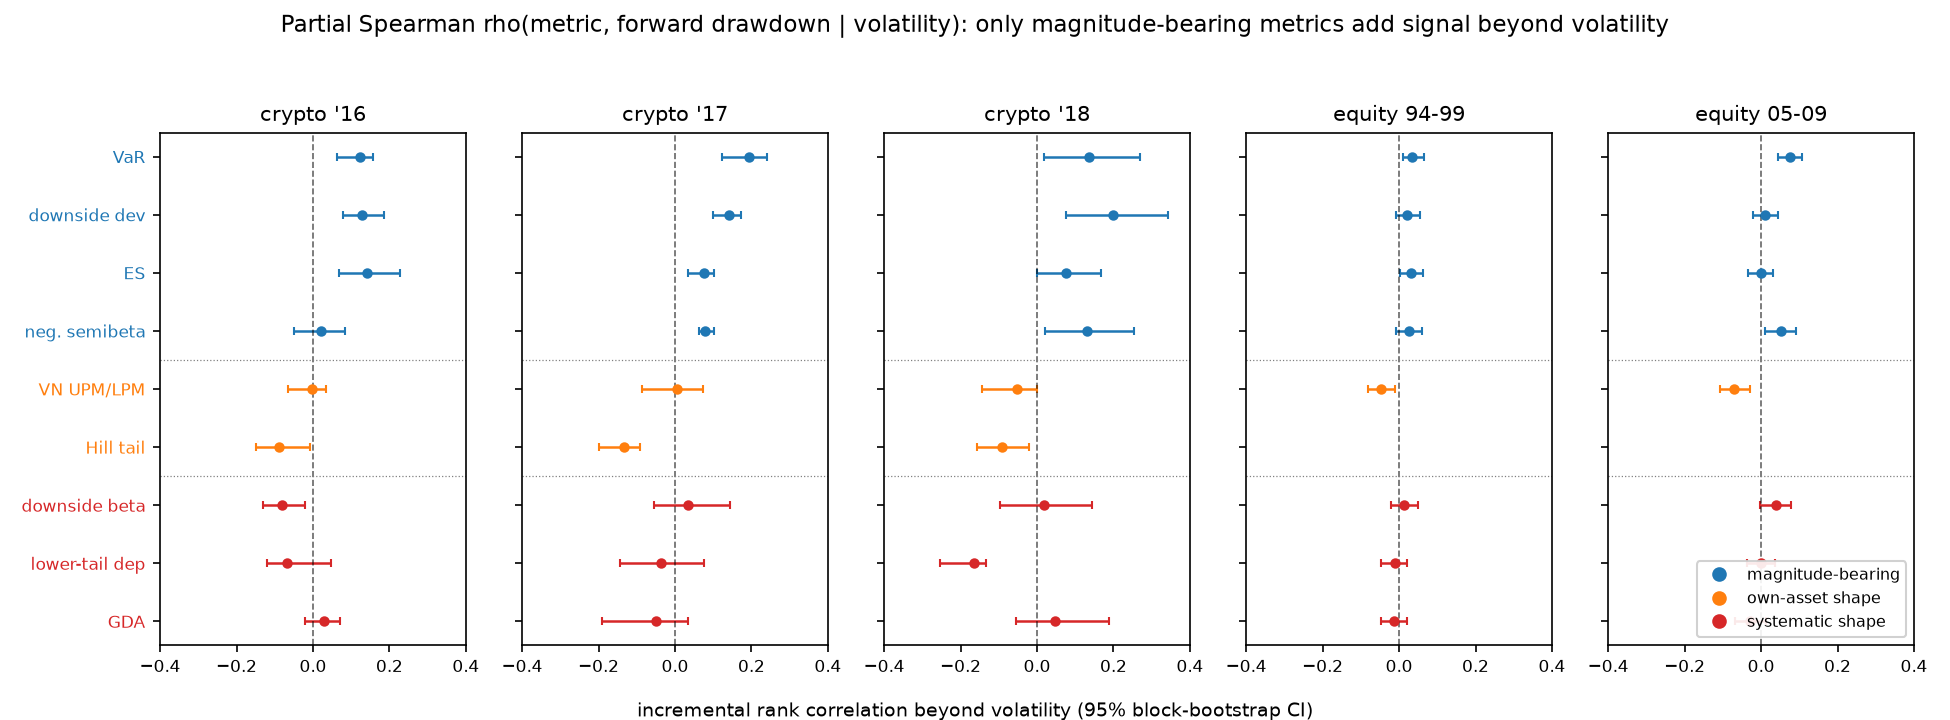
\includegraphics[width=\textwidth]{figures/fig1_partial_forest.png}
\caption{Incremental signal beyond volatility, by bed. Partial Spearman
$\rho(\text{metric},\text{drawdown}\mid\text{volatility})$, grouped by whether a metric
embeds downside magnitude. Only the magnitude-bearing metrics (blue: VaR, downside
deviation, ES, and negative semibeta, whose down-down semicovariance construction carries
downside magnitude) sit reliably right of zero. The magnitude-free shape metrics add
$\approx0$ or subtract, both the own-asset ones (orange: the Viole--Nawrocki (VN) UPM/LPM
ratio and the Hill tail exponent) and the systematic co-movement ones (red: downside beta,
lower-tail dependence, and the disappointment-aversion (GDA) proxy). Magnitude beats shape
on both sides of the own-asset/systematic divide. Whiskers are $95\%$ block-bootstrap CIs;
dotted lines separate the three groups.}
\label{fig:forest}
\end{figure*}

VaR is worse than volatility
standalone on equity (Table~\ref{tab:h2h}) yet has a positive increment there.
As a standalone ranker it is a noisier proxy for volatility, but the partial
correlation isolates its small orthogonal component. The increment is also larger where
markets are fat-tailed and blow-up-prone. Crypto increments run $0.12$--$0.19$ where excess
kurtosis is $8$--$21$, against equity increments of $0.03$--$0.08$ where kurtosis is far
lower. A pooled per-date regression of the increment on tail-fatness across all $144$ dates
gives a positive slope ($+0.013$, $95\%$ CI $[0.007,0.021]$); clustering by bed widens the
CI to $[-0.004,0.032]$ (one-sided $p=0.10$), so we read it as suggestive. Tail magnitude
carries incremental information precisely when the tail is active. When crypto dates are
split at the cross-sectional median of volatility, the increment rises from $+0.13$ on
low-stress dates to $+0.18$ on high-stress ones, while on equity it stays flat and small.

\begin{table}[t]
\centering
\caption{Partial Spearman $\rho(\text{metric},\text{drawdown}\mid\text{volatility})$.
Rows 1--3 are own-asset tail magnitude; row 4 (negative semibeta) is magnitude-bearing
through its down-down semicovariance; rows 5--9 are magnitude-free shape. $\ast$ survives
BH ($q=0.05$, positive); $\dagger$ survives BH negative; n/e = not estimable per date
(too few loss-tail observations to fit a Hill exponent per date on equity). Bold marks the
highest value in each column.}
\label{tab:partials}
\small
\begin{tabular}{lccccc}
\toprule
Metric & cr-16 & cr-17 & cr-18 & eq 94 & eq 05 \\
\midrule
VaR & $+0.12\ast$ & $\mathbf{+0.19}\ast$ & $+0.13\ast$ & $\mathbf{+0.03}\ast$ & $\mathbf{+0.08}\ast$ \\
downside dev. & $+0.13\ast$ & $+0.14\ast$ & $\mathbf{+0.20}\ast$ & $+0.02$ & $+0.01$ \\
ES~\cite{rockafellar2000} & $\mathbf{+0.14}\ast$ & $+0.08\ast$ & $+0.08$ & $\mathbf{+0.03}$ & $+0.00$ \\
neg.\ semibeta~\cite{bpq2022} & $+0.02$ & $+0.08\ast$ & $+0.13\ast$ & $\mathbf{+0.03}$ & $+0.05\ast$ \\
UPM/LPM~\cite{violenawrocki2016} & $-0.00$ & $+0.01$ & $-0.05$ & $-0.05\dagger$ & $-0.07\dagger$ \\
downside beta~\cite{ang2006} & $-0.08\dagger$ & $+0.03$ & $+0.02$ & $+0.01$ & $+0.04$ \\
Hill tail~\cite{kellyjiang2014} & $-0.09\dagger$ & $-0.13\dagger$ & $-0.09\dagger$ & n/e & n/e \\
lower-tail dep.~\cite{chabiyo2018} & $-0.07$ & $-0.04$ & $-0.17\dagger$ & $-0.01$ & $+0.00$ \\
GDA~\cite{faragotedongap2018} & $+0.03$ & $-0.05$ & $+0.05$ & $-0.01$ & $-0.03$ \\
\bottomrule
\end{tabular}
\end{table}

\begin{table}[t]
\centering
\small
\caption{VaR partial $\rho(\text{VaR},\text{drawdown}\mid\text{vol})$ under three
delisting codings. Baseline ($-100\%$) and last-price coincide (mid-window delistings are
rare); the increment is unchanged to within $\pm0.02$.}
\label{tab:delisting}
\begin{tabular}{lccc}
\toprule
Bed & baseline ($-100\%$) & last-price & exclude \\
\midrule
crypto-16 & $+0.12$  & $+0.12$  & $+0.14$  \\
crypto-17 & $+0.19$  & $+0.19$  & $+0.19$  \\
crypto-18 & $+0.14$  & $+0.14$  & $+0.14$  \\
equity-94 & $+0.035$ & $+0.035$ & $+0.035$ \\
equity-05 & $+0.076$ & $+0.076$ & $+0.076$ \\
\bottomrule
\end{tabular}
\end{table}

\subsection{Is the target the reason?}
Expected maximum drawdown scales with $\sigma\sqrt{T}$~\cite{magdonismail2004}, so
drawdown is magnitude-dominated, and one might object that a magnitude metric is bound
to win. The objection is correct, and it is the point. Drawdown is the loss that ruins
investors, and the literature proposes shape metrics to forecast it. To confirm the
shape metrics are not strawmen, we re-score every metric against genuinely
shape-sensitive forward targets, namely forward return skew (sign-flipped so higher is
more left-asymmetric), the downside fraction (forward downside deviation over forward
volatility), and the tail-exceedance frequency (share of forward days below the trailing
fifth percentile). The picture inverts (Table~\ref{tab:target}). Volatility's rank
correlation on these targets is near zero or negative, while the shape metrics beat it on
nearly every bed. Shape metrics forecast shape. Shape is simply not what drives drawdown.
The daily adaptations are therefore faithful rather than weakened. The Hill exponent is a
per-asset simplification of the Kelly--Jiang common tail factor, and the Viole--Nawrocki
ratio is high when upside dominates downside, so its zero increment beyond volatility
reflects a real null, not a wrong sign.

\begin{table}[t]
\centering
\small
\caption{Winner by forward target. Volatility wins the magnitude target; shape metrics
win every shape-sensitive target.}
\label{tab:target}
\begin{tabular}{lcc}
\toprule
Forward target & vol rank corr (range) & shape beats vol \\
\midrule
max drawdown (magnitude) & $+0.36$ to $+0.62$ & none, any bed \\
$-$skew (shape) & $-0.21$ to $-0.07$ & most, every bed \\
downside fraction (shape) & $-0.25$ to $-0.05$ & most, every bed \\
tail-exceedance freq (shape) & $-0.52$ to $-0.10$ & most, every bed \\
\bottomrule
\end{tabular}
\end{table}

%% =========================================================================
\section{Why volatility wins, and can anything beat it?}\label{sec:why}
\subsection{Persistence}
Volatility wins because it is persistent, the founding
fact of ARCH/GARCH~\cite{engle1982,bollerslev1986}. Trailing volatility forecasts
forward volatility (rank correlation $0.42$--$0.84$), which in turn drives forward
drawdown. Table~\ref{tab:chain} decomposes this chain by bed. Both links exceed the
direct trailing-vol$\rightarrow$drawdown rank correlation they compose. We resist
calling forward volatility a
\emph{sufficient statistic}. A naive same-window mediation suggests it, but that test
is contaminated (forward volatility and drawdown share a window). Measured on a
disjoint, predictive window (forward volatility over $[t,t{+}30]$ and drawdown over
$[t{+}30,t{+}120]$, so mediator and outcome share no days), trailing volatility retains a
partial correlation of $0.32$--$0.34$ on equity (Figure~\ref{fig:mediation}). Because that disjoint mediator is
a noisy $30$-day proxy, we read this as consistent with incomplete mediation rather than
proof, so persistence is a leading but incomplete explanation, not a mechanism that
reduces drawdown to one number.

\begin{table}[t]
\centering
\caption{Persistence chain (mean per-date Spearman; dd = drawdown; all CIs exclude 0).}
\label{tab:chain}
\small
\begin{tabular}{lccc}
\toprule
Bed & trail$\rightarrow$fwd vol & fwd vol$\rightarrow$dd & (trail$\rightarrow$dd) \\
\midrule
crypto-16 & 0.68 & 0.77 & 0.62 \\
crypto-17 & 0.42 & 0.62 & 0.36 \\
crypto-18 & 0.42 & 0.53 & 0.38 \\
equity 94 & 0.84 & 0.71 & 0.61 \\
equity 05 & 0.80 & 0.70 & 0.56 \\
\bottomrule
\end{tabular}
\end{table}

\begin{figure}[t]
\centering
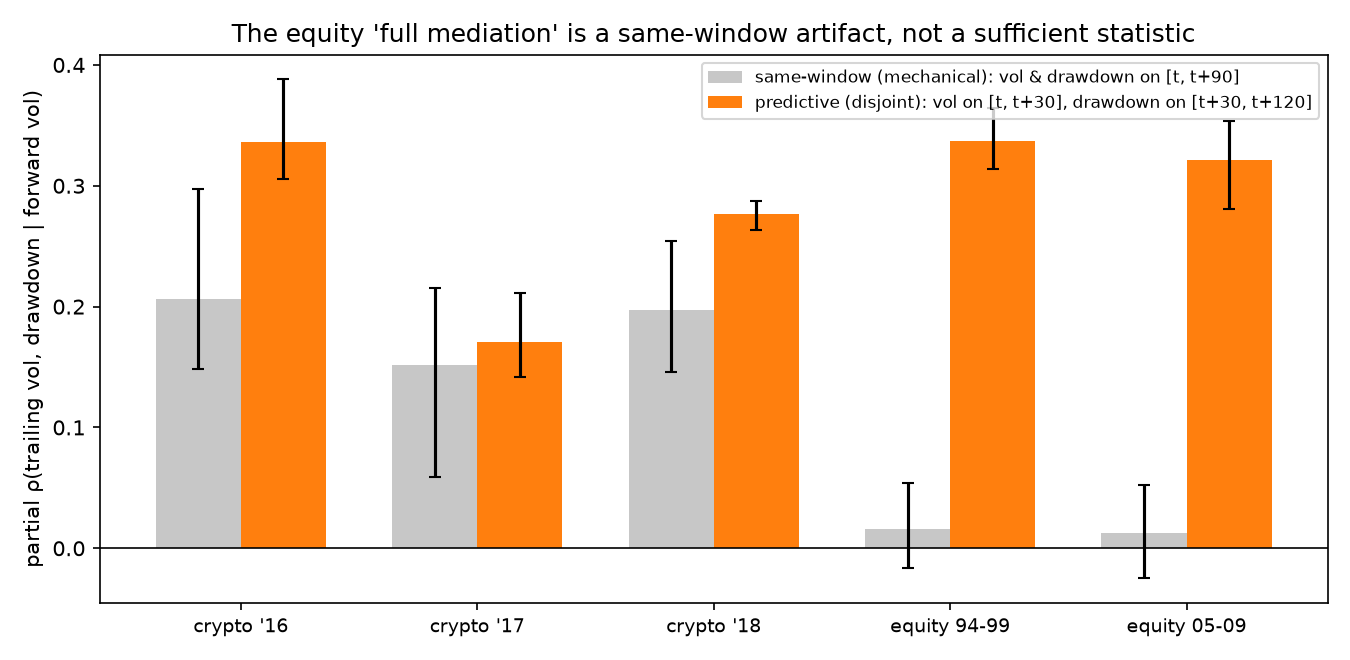
\includegraphics[width=\columnwidth]{figures/fig3_mediation.png}
\caption{Mediation: partial $\rho(\text{trailing vol},\text{drawdown}\mid
\text{forward vol})$. The same-window (mechanical) design gives $\approx 0$ on equity,
falsely suggesting full mediation. The predictive (disjoint-window) design gives
$0.32$--$0.34$, so forward volatility does not fully screen off trailing volatility.}
\label{fig:mediation}
\end{figure}

\textbf{Horizon dynamics.} Persistence and forecastability rise and fall together. As we
sweep the forecast horizon from $14$ to $90$ days, volatility persistence and the drawdown
rank correlation move in step (Figure~\ref{fig:horizon}). On equity both rise (persistence
$0.66\rightarrow0.84$, rank correlation $0.47\rightarrow0.61$) at a roughly constant gap,
while on crypto both are flat. Wherever persistence is higher, so is the rank correlation,
consistent with persistence driving most of the forecastable variation and the constant
gap being the part it does not explain.

\begin{figure*}[t]
\centering
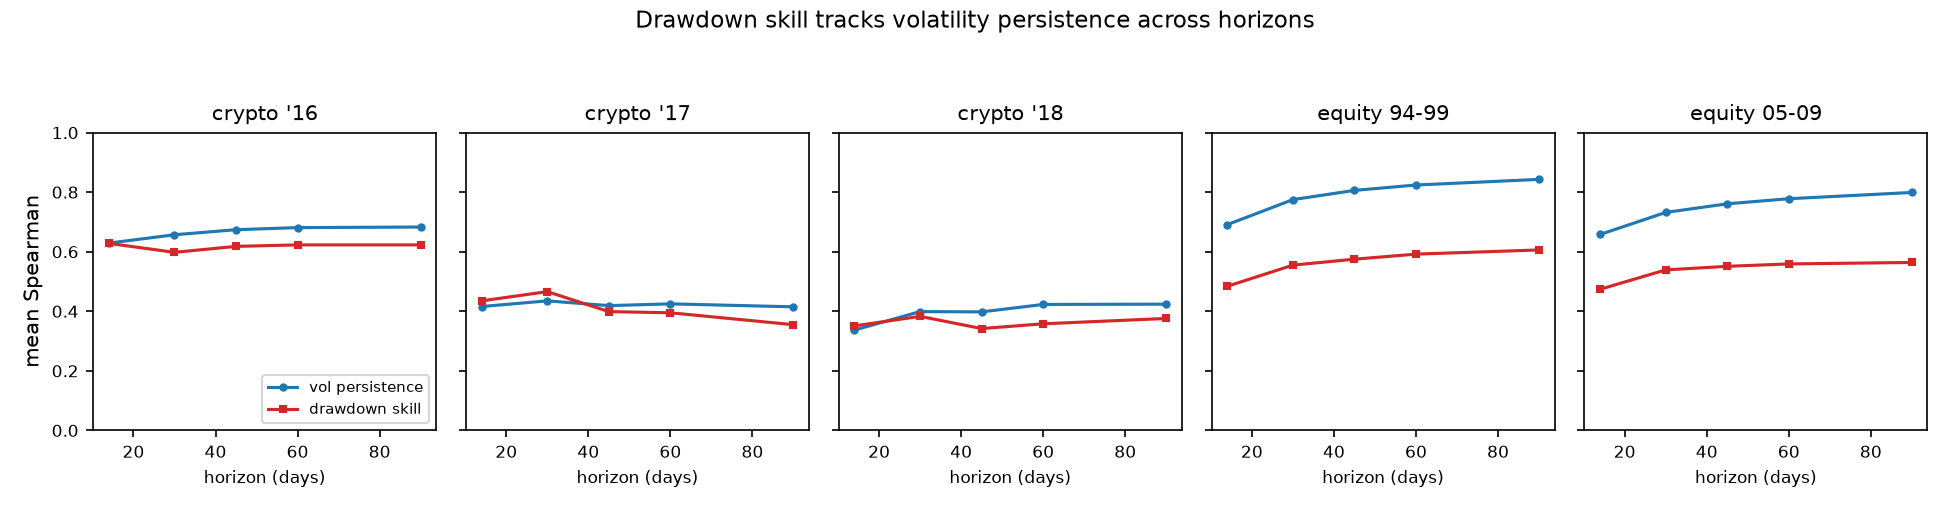
\includegraphics[width=\textwidth]{figures/fig4_horizon_decay.png}
\caption{Volatility persistence (blue) and drawdown-forecast rank correlation (red) versus
forecast horizon ($14$--$90$ days), by bed. The two curves rise and fall together at a
roughly constant gap, so where volatility is more persistent it also forecasts drawdown
better.}
\label{fig:horizon}
\end{figure*}

\subsection{Does the edge pay?}
A rank correlation is not a profit-and-loss statement.
The magnitude-not-shape split of \S\ref{sec:magnitude}, volatility plus a single
tail-magnitude term, implies one natural composite, the equal-weight sum
$z(\text{vol})+z(\text{VaR})$ with no fitting, where $z(\cdot)$ is the cross-sectional
z-score (each metric standardized across the assets on a given date). VaR was fixed as the
composite's second term before the locked panel was opened. It was the only metric whose
increment survived correction on all five exploratory beds, and the weights are untuned,
so the locked panel is fully out-of-sample. There it shows no significant out-of-sample
gain over volatility (Newey--West $t=0.67$, lag $3$), beating it only on fat-tailed
crypto-bull (Table~\ref{tab:econ}). That crypto-bull edge is $+0.05$, below the bed's
$80\%$-power MDE of $0.09$, so like VaR's crypto claims it is suggestive rather than
powered. A cost-aware tercile backtest agrees (Figure~\ref{fig:economic}). The
high-risk tercile realizes $10$--$30$ percentage points more forward drawdown than the
low-risk tercile on every bed, net of a $20$-basis-point (bps) cost charged on portfolio
turnover at each rebalance (terciles, rebalanced per formation date), and the composite
adds nothing net of turnover except, again, on crypto-bull. Volatility is the workhorse.
Magnitude adds a little, and only where tails are fat.

\begin{table}[t]
\centering
\caption{Composite $z(\text{vol})+z(\text{VaR})$ vs.\ volatility, per-date Spearman
and difference (95\% CI). The difference is significantly positive only on crypto-bull and
significantly negative, though trivially small, on equity-94; n.s.\ = not significant (the
difference's $95\%$ CI includes $0$). The locked panel trains on $2017$ and is scored once
on the $2018$ crash.}
\label{tab:econ}
\small
\begin{tabular}{lccc}
\toprule
Test bed & vol $\rho$ & comp $\rho$ & difference (95\% CI) \\
\midrule
crypto-16 & 0.62 & 0.62 & $-0.00$ (n.s.) \\
crypto-17 & 0.36 & 0.40 & $+0.05$ $[0.02,0.07]$ \\
crypto-18 & 0.38 & 0.39 & $+0.01$ (n.s.) \\
equity 94 & 0.61 & 0.60 & $-0.008$ $[-0.011,-0.004]$ \\
equity 05 & 0.56 & 0.56 & $-0.00$ (n.s.) \\
\midrule
\multicolumn{4}{l}{\emph{Locked panel:} $0.376 \rightarrow 0.388$, Newey--West $t=0.67$ (n.s.).}\\
\bottomrule
\end{tabular}
\end{table}

\begin{figure}[t]
\centering
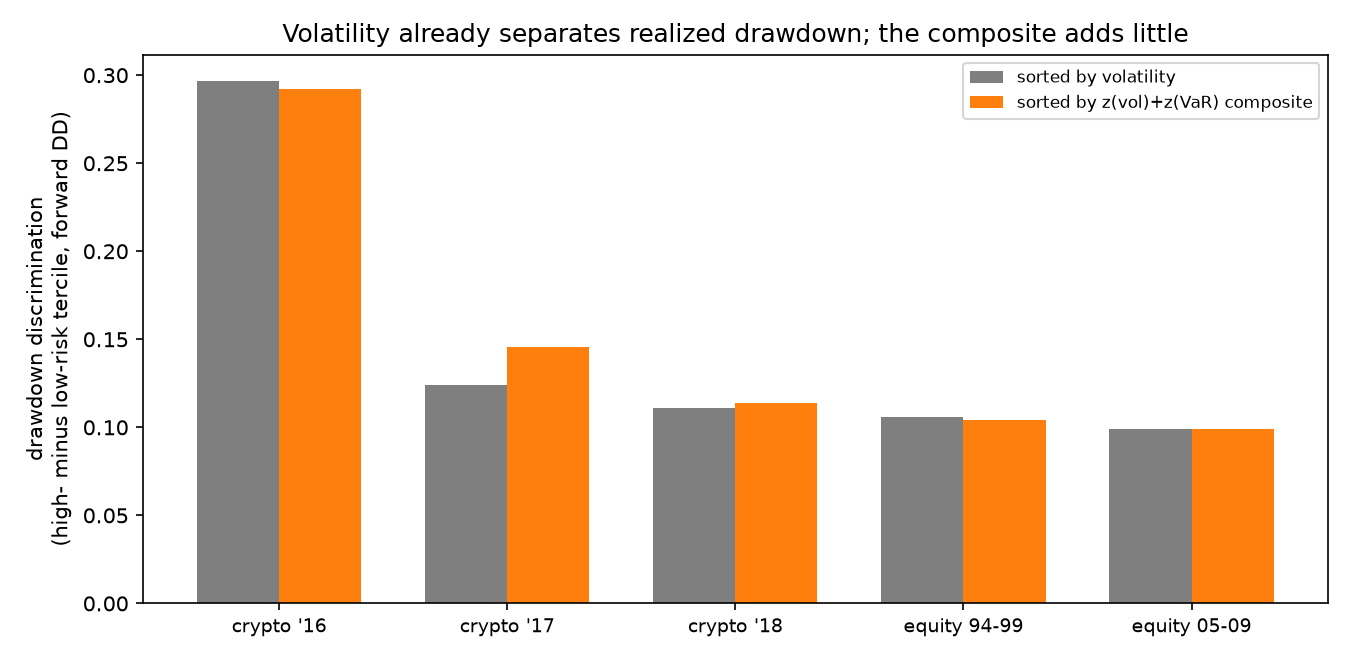
\includegraphics[width=\columnwidth]{figures/fig7_economic.png}
\caption{Realized drawdown discrimination (high minus low-risk tercile) by bed, sorting on
volatility vs.\ the composite. Volatility already separates drawdown strongly; the
composite is indistinguishable except marginally on crypto-bull.}
\label{fig:economic}
\end{figure}

\subsection{Can a machine find more?}
If the residual is this small, a tireless automated
search should fail out-of-sample and merely overfit validation. We test this on a strict
train/validation/locked-test split, the locked test scored once after the metric
is frozen. On the original locked panel, an LLM agent rewriting a scoring function and a
$20{,}000$-configuration sweep both inflate the best \emph{validation} score with search
intensity while the \emph{locked-test} score plateaus at the volatility baseline
(Table~\ref{tab:bon}, Figure~\ref{fig:bon}). Of the swept configurations that beat
volatility on validation, only $43\%$ also beat it on the locked test, despite a $0.94$
validation--test rank correlation.

\textbf{The discovery loop.} The agent is Claude Opus 4.8. It is given a frozen scorer it
may not edit, a train/validation split, and a single file defining
\texttt{build\_scores(panel)}. Each iteration it reads the log of past attempts and the
current metric, rewrites the metric with one new idea (any Python over the per-row features
volatility, ES, VaR, LPM$_2$, downside deviation, trailing drawdown, skew, kurtosis, and
market cap, fitting any parameters on the train split only), scores it on validation, and
keeps the edit if validation improved, otherwise reverts. It never sees the locked test,
which a separate frozen script scores exactly once after the metric is finalized. The run
we report ran $51$ iterations ($14$ kept, $37$ discarded), lifting validation from $0.31$
to $0.34$. The $20{,}000$-configuration sweep enumerates the same feature-combination space
(sums, ratios, products, gates, interactions) exhaustively, and the general nonlinear
generator samples $1{,}500$ such candidates per run. All three optimize the same validation
score against the same locked test.

\begin{table}[t]
\centering
\caption{Best-of-$N$ discovery on the original locked panel. Validation inflates with
search intensity; the locked test does not (volatility baseline $0.376$). Validation and
test are different splits, so compare trends, not levels.}
\label{tab:bon}
\small
\begin{tabular}{rcc}
\toprule
Search intensity $N$ & Best validation & Its locked test \\
\midrule
1 & 0.27 & 0.31 \\
100 & 0.35 & 0.37 \\
20{,}000 & 0.356 & 0.373 \\
\bottomrule
\end{tabular}
\end{table}

This is not a single-panel artifact. We re-ran a general nonlinear candidate generator
($1{,}500$ candidates per run) across a grid of holdout panels $\times$ $3$ search seeds
in two families: \emph{out-of-time}, a fixed-length test window slid through the timeline
with validation always chronologically earlier; and \emph{random}, order-ignoring
repartitions of the non-train dates. The validation-selected metric's locked-test edge over
volatility (test gap) is small but positive, averaging $+0.020$ out-of-time (clustered
$t=4.3$ across the six panels) and $+0.035$ under random repartitions ($t=5.3$), while the
validation--test rank correlation stays $0.94$--$0.99$ throughout. Two readings follow.
First, the out-of-time edge is tiny and consistent with search rediscovering the same
tail-magnitude increment of \S\ref{sec:magnitude}, not new signal. Second, the random-split
edge is the larger of the two, a signature of temporal leakage, because order-ignoring
repartitions interleave validation and test dates and let volatility's persistence leak
across the split, manufacturing a phantom edge. Only chronological holdouts are honest in
persistent panels. Either way the edge is economically negligible, and the non-LLM sweep
reproduces it, so the danger is the cheap search, not the language model.

The statistics are classical data snooping~\cite{white2000,bailey2017}. What is new is
that an autonomous agent removes the last brake on trial count, namely analyst effort, so
a locked, survivorship-free holdout scored exactly once becomes mandatory, not merely
advisable.

\subsection{What is volatility for?}
The clearest positive use is forecasting outright
blow-ups. On the locked crypto test, volatility predicts which assets crater (forward
return $\le -80\%$) with ROC-AUC $0.68$ ($0.95$
for the stricter $\le -90\%$ cutoff) and a $2.5\times$
top-decile lift, while a gradient-boosting model over all ten metrics, chosen on
validation (AUC $0.73$), overfits and loses on the locked test (AUC $0.59$). The
blow-up base rate is only ${\approx}1.2\%$, so these AUCs are noisy and we read them as
ordinal. Again the size, not the shape, of recent moves carries the
signal. This is a ranking result, not a deployment recommendation (cost, liquidity, and
reflexivity frictions are unmodeled).

\begin{figure*}[t]
\centering
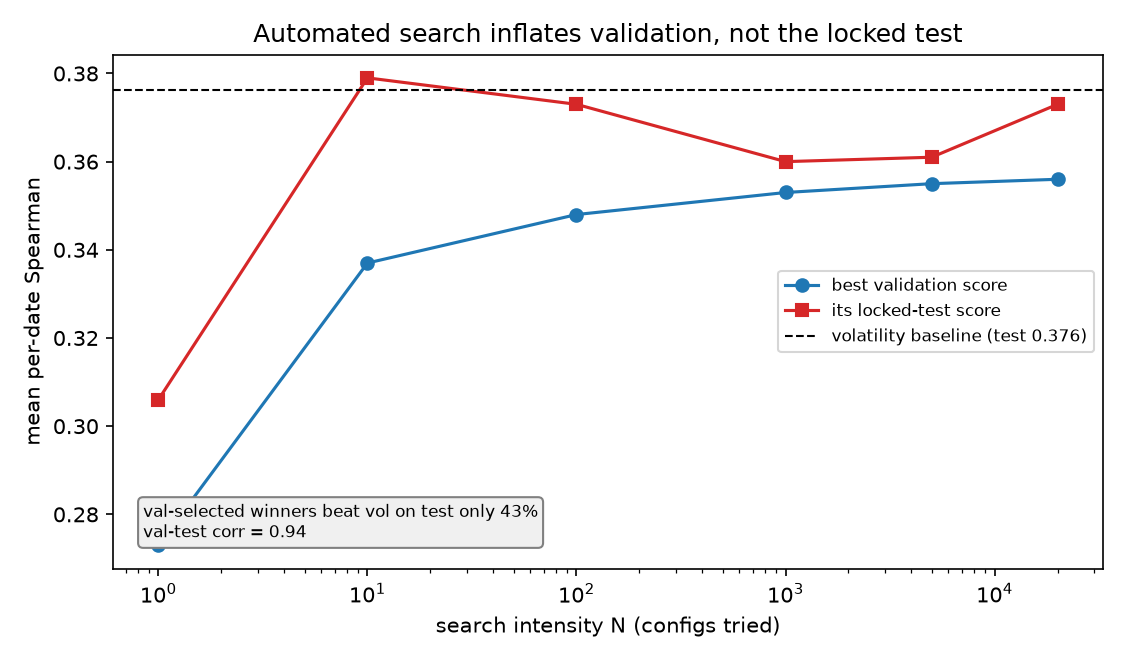
\includegraphics[width=0.7\textwidth]{figures/fig5_best_of_N.png}
\caption{Automated discovery does not beat volatility out of sample by more than a sliver.
As search intensity grows, the best validation score climbs while its locked-test score
stays flat at the volatility baseline. On this ($2017\!\to\!2018$-crash) holdout, only
$43\%$ of the configurations that beat volatility on validation also beat it on the locked
test. Across $12$ panels $\times$ $3$ seeds the locked-test edge is statistically positive
but economically negligible ($+0.02$ out-of-time), and larger under order-ignoring random
splits, the signature of temporal leakage.}
\label{fig:bon}
\end{figure*}

%% =========================================================================
\section{How much do the disciplines matter?}\label{sec:ablation}
The three fair-field disciplines change what one would report, not the verdict. We ask
which shape metric one would have credited without each.

\textit{Without survivorship-free data.} We rebuild the crypto universe survivors-only,
keeping at each formation date only coins that neither delisted nor ended below $5\%$ of
their all-time peak, about a third of the point-in-time top $100$. On the $2018$ crash
bed this erases shape's penalty and inflates the magnitude edge (Table~\ref{tab:ablation}).
Negative semibeta, a co-crash shape metric, flips from significantly worse than volatility
to a tie, downside beta closes its gap, and VaR's partial rises. This happens precisely in
the crash regime, where hiding the coins that died most reshapes the cross-section. It does
not manufacture a winner. No shape metric beats volatility even survivors-only.

\begin{table}[t]
\centering
\small
\caption{Survivorship ablation on the crypto-2018 crash bed, vs.\ volatility (block-bootstrap
$95\%$ CIs where estimated). Dropping the coins that died turns a co-crash shape metric's loss
into a tie and inflates the magnitude edge, yet no shape metric beats volatility either way.}
\label{tab:ablation}
\setlength{\tabcolsep}{3.5pt}
\begin{tabular}{lcc}
\toprule
crypto-2018 & full universe & survivors-only \\
\midrule
neg.\ semibeta (h2h) & $-0.067\,[\text{-}0.131,\text{-}0.003]$ & $+0.055\,[\text{-}0.082,0.178]$ \\
downside beta (h2h) & $-0.23$ & $-0.01$ \\
VaR (partial $\rho$) & $+0.135$ & $+0.205$ \\
\bottomrule
\end{tabular}
\end{table}

\textit{Without multiple-testing correction.} Across the ${\sim}45$ head-to-head cells the
only metrics nominally beating volatility at $p<0.05$ are downside deviation and VaR,
both magnitude measures, and only on crypto-bull. No shape metric is even nominally
positive, so Benjamini--Hochberg is not what holds shape back.

\textit{Without a locked holdout.} The discovery experiment (\S\ref{sec:why},
Table~\ref{tab:bon} and Figure~\ref{fig:bon}) makes this concrete. A validation-selected metric's inflated validation score reads as a win, while
its once-scored locked-test score sits at the volatility baseline. Even stripped of every
guardrail, no shape metric beats volatility.

%% =========================================================================
\section{Discussion and conclusion}\label{sec:discussion}
The pieces form one coherent picture. Volatility sets a high bar because it is
persistent (\S\ref{sec:why}). The only thing left to add is the magnitude of tail
losses, and only a little, mostly in fat-tailed markets (\S\ref{sec:magnitude}). So no
standalone metric beats volatility (\S\ref{sec:verdict}), a pre-registered composite
yields no significant out-of-sample gain, automated search cannot find one, and the
economics track the statistics (\S\ref{sec:why}). The recurring
failure of magnitude-free asymmetry and shape
metrics (including the partial-moment ratio~\cite{violenawrocki2016}) is
not an implementation accident. Once symmetric volatility is accounted for, asymmetric
structure adds incremental cross-sectional information for forecasting drawdown only when
it also carries downside magnitude, as in negative semibeta; pure shape adds nothing. The fair-field disciplines change what one would report, not the
verdict (\S\ref{sec:ablation}). Survivorship bias alone flips a co-crash shape metric
from significantly worse than volatility to a tie and inflates the apparent magnitude
edge, yet the verdict that no shape metric beats volatility is robust to dropping any
single discipline. The disciplines guard the honesty of the numbers, not the direction
of the conclusion.

We are deliberately careful about the strength of the
persistence story. An earlier version of this study claimed forward volatility
was a sufficient statistic, found that claim was a same-window measurement
artifact, and corrected it in this version, just as an earlier ``survivorship masks
downside value'' thesis was dropped when a hardened test refuted it. The paper
reports only claims that survived stress-testing.

The practical takeaway is plain but firm. For cross-sectional drawdown
forecasting, use volatility (optionally with a small tail-magnitude term in
fat-tailed markets) and treat any downside metric ``discovered'' to beat it,
by hand or by machine, as unproven until it clears a locked, survivorship-free
holdout. On a level field, volatility is not glamorous, but it is very hard to beat.

\textbf{Limitations.} The performance measure is rank correlation, not a full tradable P\&L
(\S\ref{sec:why} is a first economic check, not a portfolio study); the
crypto beds have few formation dates ($7$--$9$), so their significance is
suggestive and the null ``shape adds nothing'' leans on the well-powered equity
beds; the trailing window is fixed at $180$ days and the horizon sweep varies only the
forward side, so sensitivity to the trailing length is unexamined; and the repurposed
pricing metrics are daily adaptations, so results speak to
drawdown forecasting, not the originals' pricing claims.

%% =========================================================================
\bibliographystyle{ACM-Reference-Format}
\bibliography{references}

\end{document}
